\documentclass[12pt]{article}
\usepackage{pgfgantt}
\usepackage{geometry} % to change margins

\begin{document}

\section*{Introducción}

El trabajo de tesis se ha desarrollado en base al objetivo general de desarrollar modelos de identificación de galaxias con entrada de imágenes multiresolución estudiando el desempeño, tanto en velocidad de procesamiento como en correctitud en la tarea a resolver. Dado lo anterior el trabajo se ha divido en las siguientes etapas.
\begin{enumerate}
    \item Estudiar y replicar resultados de DELIGHT \cite{delight} bajo framework original (TensorFlow)
    \item Explorar y replicación del modelo convolucional usando el framework Torch y comparar desempeño de ambas redes midiendo tanto eficiencia en cómputo en la ejecución de la red, como eficacia a la hora de resolver la tarea.
    \item Explorar la confección de modelo basado en Vision Transformers (ViT) partiendo con imágenes de resolución simple y comparar desempeño respecto a las redes desarrolladas anteriormente. \cite{DBLP:journals/corr/abs-2010-11929}.
        \begin{itemize}
            \item En función de si el modelo resultante tenga mejor desempeño que sus contrapartes convolucionales, se buscará incorporar imágenes multiresolución y comparar desempeño. En caso contrario, se optimizará la arquitectura e hiperparámetros
        \end{itemize}
    \item Explorar incorporación de información de varias bandas, esto es, comparar desempeño utilizando imágenes multiresolución de varios canales.
    \item Explorar extensiones a otras aplicaciones, e.g. clasificación de imágenes en google maps usando imágenes multi resolución.
\end{enumerate}

Las cuales se encuentran resumidas en la carta gantt anexada. Se espera terminar el trabajo propuesto junto con el manuscrito a finales de Junio 2024 y, a su vez, se contempla el mes de Julio 2024 para atrasos en la agenda.

\mbox{}
\vfill
\begin{center}
\begin{tabular}{ c c c }
 \line(1,0){100} & \line(1,0){120} & \line(1,0){130} \\ 
 Firma Estudiante & Firma profesor(a) guía & Firma profesor(a) coguía     
\end{tabular}
\end{center}

\newpage

\tikzset{
   oddlines/.style={
        line width=\ganttvalueof{y unit chart},
        yshift=-0.5*\ganttvalueof{y unit chart},
        opacity=0.2,
        red
   },
  evenlines/.style={
      oddlines,
      blue
  }
}

\noindent\resizebox{\textwidth}{!}{
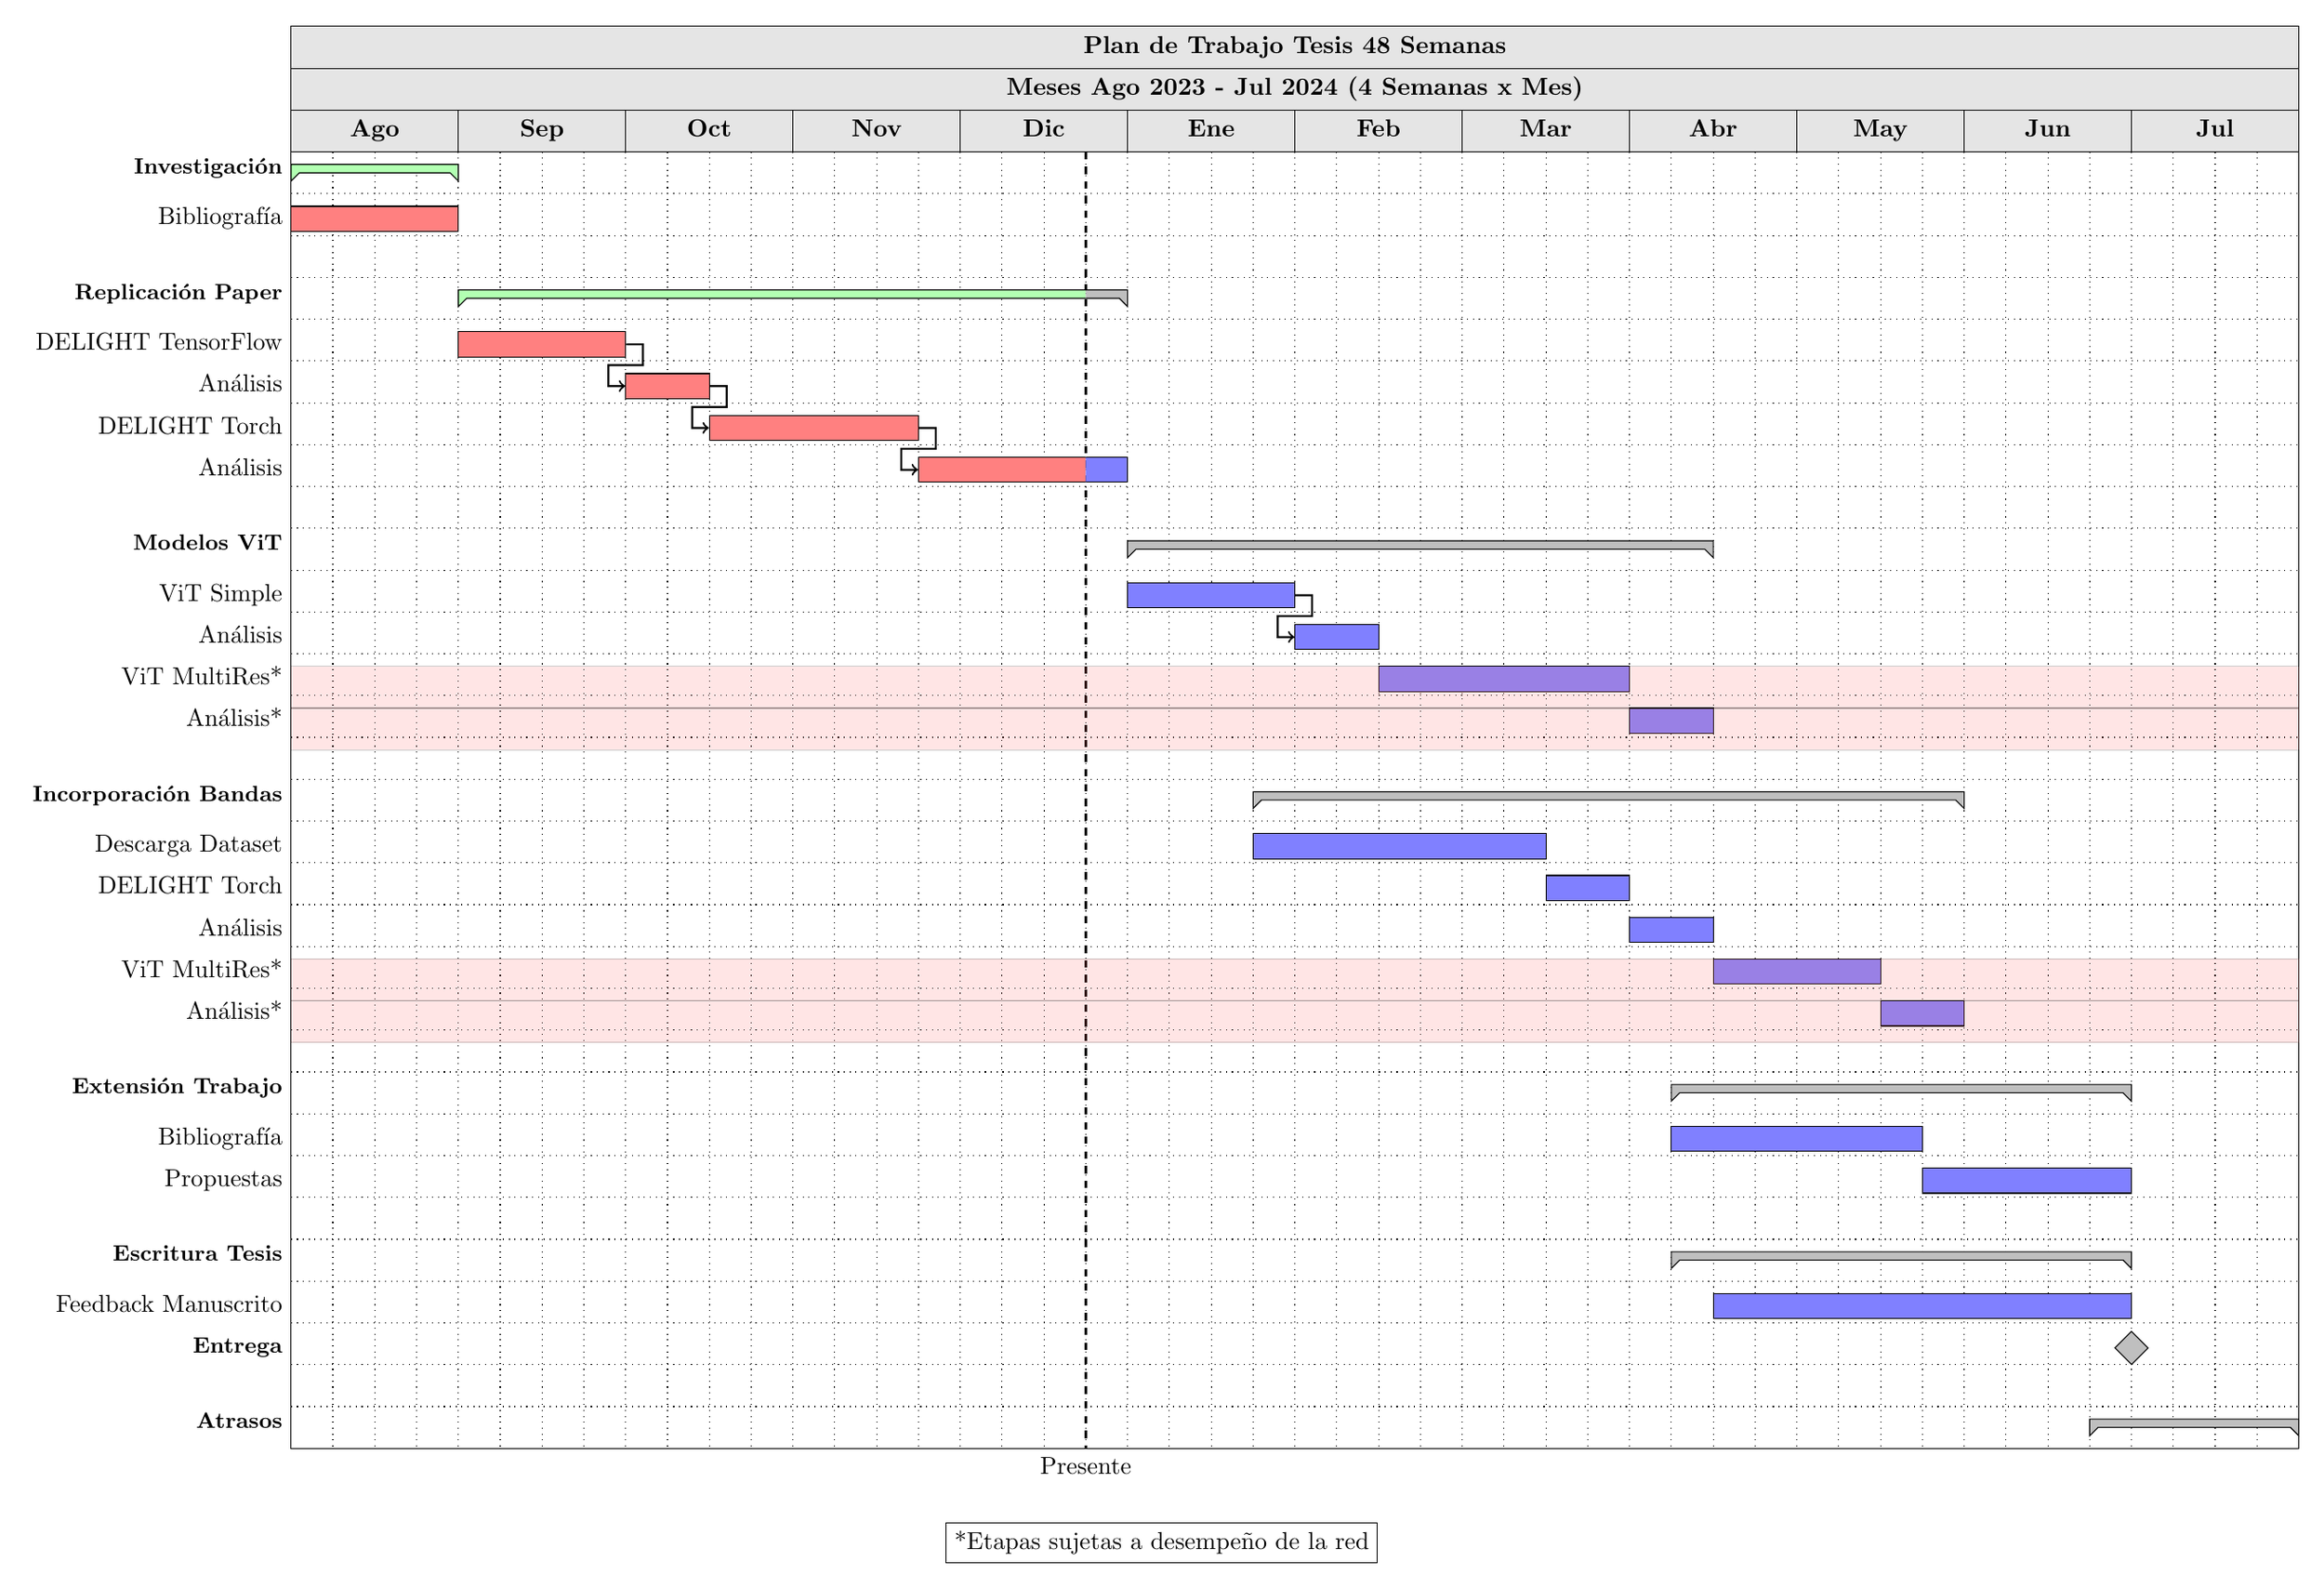
\begin{tikzpicture}[x=.3cm, y=1cm]
\begin{ganttchart}[
    vgrid,
    hgrid,
    x unit=0.6cm,
    y unit title=0.6cm,
    y unit chart=0.6cm,
    title/.append style={fill=gray!20},
    title label font=\bfseries,
    title height=1,
    bar height=0.6,
    bar/.append style={fill},
    bar incomplete/.append style={fill=blue!50},
    bar/.append style={fill=red!50},
    progress label text={},
    milestone label font=\bfseries\small,
    milestone height=0.8,
    milestone top shift=0.2,
    milestone/.append style={fill=red},
    group/.append style={draw=black, fill=green!30},
    group height=.3,
    group peaks height=.2,
    group label font=\bfseries\small,
    group left shift=0,
    group right shift=0,
    group top shift=.3,
    group height=.2,
    group peaks tip position=0,
    group peaks width=0.2,
    group incomplete/.append style={fill=gray!50},
    link/.style={->,thick},
    expand chart=20cm,
    today=19,
    today label=Presente,
    progress=today,
    % inline
    ]{1}{48}

    \gantttitle{Plan de Trabajo Tesis 48 Semanas}{48} \\
    \gantttitle{Meses Ago 2023 - Jul 2024 (4 Semanas x Mes)}{48} \\
    \gantttitle{Ago}{4}
    \gantttitle{Sep}{4}
    \gantttitle{Oct}{4}
    \gantttitle{Nov}{4}
    \gantttitle{Dic}{4} 
    \gantttitle{Ene}{4} 
    \gantttitle{Feb}{4} 
    \gantttitle{Mar}{4} 
    \gantttitle{Abr}{4} 
    \gantttitle{May}{4}
    \gantttitle{Jun}{4}
    \gantttitle{Jul}{4} \\
    
    \ganttgroup{Investigación}{1}{4} \\ 
    \ganttbar{Bibliografía}{1}{4} \\ \\
    
    \ganttgroup{Replicación Paper}{5}{20} \\
    \ganttbar{DELIGHT TensorFlow}{5}{8} \\
    \ganttlinkedbar{Análisis}{9}{10} \\
    \ganttlinkedbar{DELIGHT Torch}{11}{15} \\
    \ganttlinkedbar{Análisis}{16}{20} \\ \\
    
    \ganttgroup{Modelos ViT}{21}{34} \\
    \ganttbar{ViT Simple}{21}{24} \\
    \ganttlinkedbar{Análisis}{25}{26} \\
    \ganttbar{ViT MultiRes*}{27}{32}
    \ganttbar[
        bar height=1,
        bar/.append style={fill=red!50, opacity=0.2},
        bar incomplete/.append style={fill=red!50, opacity=0.2},
    ]{}{1}{48} \\
    \ganttbar{Análisis*}{33}{34}
    \ganttbar[
        bar height=1,
        bar/.append style={fill=red!50, opacity=0.2},
        bar incomplete/.append style={fill=red!50, opacity=0.2},
    ]{}{1}{48} \\ \\

    \ganttgroup{Incorporación Bandas}{24}{40} \\
    \ganttbar{Descarga Dataset}{24}{30} \\
    \ganttbar{DELIGHT Torch}{31}{32} \\
    \ganttbar{Análisis}{33}{34} \\
    \ganttbar{ViT MultiRes*}{35}{38} 
    \ganttbar[
        bar height=1,
        bar/.append style={fill=red!50, opacity=0.2},
        bar incomplete/.append style={fill=red!50, opacity=0.2},
    ]{}{1}{48} \\
    \ganttbar{Análisis*}{39}{40}
    \ganttbar[
        bar height=1,
        bar/.append style={fill=red!50, opacity=0.2},
        bar incomplete/.append style={fill=red!50, opacity=0.2},
    ]{}{1}{48} \\ \\

    \ganttgroup{Extensión Trabajo}{34}{44} \\
    \ganttbar{Bibliografía}{34}{39} \\
    \ganttbar{Propuestas}{40}{44} \\ \\
    
    \ganttgroup{Escritura Tesis}{34}{44} \\
    \ganttbar{Feedback Manuscrito}{35}{44} \\
    \ganttmilestone{Entrega}{44} \\ \\
    \ganttgroup{Atrasos}{44}{48}

    \node[fill=white,draw] at ([yshift=-40pt]current bounding box.south){*Etapas sujetas a desempeño de la red};

\end{ganttchart}
\end{tikzpicture}
}

\newpage

\bibliographystyle{apalike} 
\bibliography{cites}

\end{document}